\section{Features Selection}\label{sec:fs} 

A \textbf{Seleção de Atributos} (\textit{Feature Selection} - FS) é reconhecida como uma etapa fundamental de pré-processamento no campo do Aprendizado de Máquina (AM) e da Mineração de Dados, particularmente em cenários que envolvem conjuntos de dados de alta dimensionalidade \cite{Dhal2022} \cite{BARBIERI2024123667} \cite{10.1007/978-3-031-23092-9_12}. Sua essência reside na busca por um subconjunto ótimo de atributos relevantes e não redundantes a partir do conjunto original, com o objetivo primário de manter ou, idealmente, aprimorar o desempenho preditivo do modelo de AM, ao mesmo tempo que se reduz a complexidade \cite{Theng2024} \cite{Emmoh2024}.

A relevância da FS é amplificada pela crescente ubiquidade de Big Data e dados de alta dimensão, que frequentemente apresentam problemas como a \textbf{maldição da dimensionalidade} (\textit{curse of dimensionality}) \cite{Dhal2022} \cite{BARBIERI2024123667} \cite{10.1007/978-3-031-23092-9_12}. Este fenômeno descreve como o espaço de dados se torna esparso à medida que o número de dimensões (atributos) aumenta, exigindo exponencialmente mais dados para manter a mesma densidade de amostragem. Além disso, a alta dimensionalidade introduz atributos irrelevantes ou redundantes que podem degradar o desempenho do classificador, aumentar o custo computacional e dificultar a interpretabilidade \cite{EBRAHIMIWARKIANI2025129372} \cite{Bouchlaghem2022}.

Ao mitigar esses desafios, a FS oferece benefícios fundamentais para o desenvolvimento de modelos de AM mais eficientes e performáticos:

\begin{itemize} \item \textbf{Redução da Complexidade e Custo Computacional:} A diminuição do número de atributos acelera significativamente o tempo de treinamento e teste dos algoritmos de AM, além de reduzir os requisitos de armazenamento \cite{Theng2024}. \item \textbf{Melhoria da Acurácia e Prevenção de \textit{Overfitting}:} Ao remover atributos ruidosos e irrelevantes, a FS permite que o modelo se concentre nas características mais discriminativas, resultando em maior poder de generalização e prevenindo o ajuste excessivo aos dados de treinamento \cite{Dhal2022}. \item \textbf{Aumento da Interpretabilidade e Descoberta de Conhecimento:} Um subconjunto menor de atributos essenciais facilita a compreensão do modelo e dos dados subjacentes por especialistas do domínio, transformando a FS em uma ferramenta de descoberta de conhecimento \cite{Dhal2022} \cite{KHAIRE20221060}. \item \textbf{Estabilidade do Algoritmo:} Em contextos de alta dimensionalidade, a estabilidade do algoritmo de FS a robustez das preferências de atributos selecionados a pequenas perturbações na amostra de treinamento é um fator tão importante quanto a acurácia de classificação. A alta correlação entre atributos pode levar a múltiplas assinaturas ótimas, tornando a estabilidade um desafio central na pesquisa de FS \cite{KHAIRE20221060}. \end{itemize}

A FS é uma área de pesquisa dinâmica e bem estabelecida, com os métodos de seleção de atributos sendo tradicionalmente categorizados em três abordagens principais: \textbf{Filtro} (\textit{Filter}), \textbf{Wrapper} e \textbf{Embedded}. Recentemente, as abordagens \textbf{Híbridas} ganharam destaque por combinarem as vantagens das técnicas anteriores \cite{EBRAHIMIWARKIANI2025129372} \cite{10895909}\cite{Theng2024} \cite{SolorioFernandez2020} \cite{10.1007/978-3-031-23092-9_12}. A escolha da abordagem de FS é um ponto crítico, pois ela influencia diretamente a estabilidade do subconjunto de atributos selecionados e o desempenho final do modelo de Aprendizado de Máquina \cite{KHAIRE20221060} \cite{BARBIERI2024123667}.



\subsection{Métodos de Filtro (Filter Methods)}
\label{subsec:filter_methods}

Os métodos de \emph{Filtro} constituem a abordagem mais simples e computacionalmente eficiente para a seleção de atributos (\emph{Feature Selection} — FS). Estes métodos atuam como etapa de pré-processamento e são inteiramente independentes do algoritmo de aprendizagem que será utilizado posteriormente. \cite{Theng2024,Dhal2022,EBRAHIMIWARKIANI2025129372,10.1007/978-3-031-23092-9_12}

\subsubsection*{Princípio de funcionamento.}
A essência dos métodos de filtro reside na aplicação de uma métrica estatística ou de teoria da informação para avaliar a relevância de cada atributo com base nas suas propriedades intrínsecas \cite{Theng2024,SolorioFernandez2020,Bouchlaghem2022}. O processo de seleção tipicamente envolve duas etapas:
\begin{enumerate}
    \item \textbf{Ranqueamento:} os atributos são pontuados individualmente (métodos univariados) ou avaliados de forma conjunta (métodos multivariados) segundo um critério, como correlação, entropia ou importância baseada em instâncias \cite{Bouchlaghem2022, geng2007feature}.
    \item \textbf{Seleção:} o subconjunto final é obtido escolhendo os atributos com maior pontuação, mediante um limiar (\emph{threshold}) ou um tamanho de subconjunto predefinido \cite{Theng2024,jovic2015review}.
\end{enumerate}


Os filtros selecionam \emph{features} com base em qualidades intrínsecas, independentemente do método de aprendizagem subsequente \cite{EBRAHIMIWARKIANI2025129372}.

\bigskip
A seleção do método de filtro deve ponderar as características do conjunto de dados e os objetivos da tarefa \cite{Theng2024}.

\begin{description}
    \item[\textbf{Vantagens}] 
    \begin{itemize}
        \item \textbf{Velocidade e eficiência computacional:} métodos de filtro apresentam baixo custo computacional e são adequados para manipulação de grandes volumes de dados. \cite{Theng2024,Dhal2022}
        \item \textbf{Escalabilidade:} apropriados para datasets de alta dimensionalidade por serem, em muitos casos, lineares ou quase lineares no custo computacional. \cite{Dhal2022,bolon2018scalability}
        \item \textbf{Independência do modelo e generalização:} por não dependerem do classificador, podem ser reutilizados com diversos modelos e tendem a reduzir viés de ajuste específico. \cite{EBRAHIMIWARKIANI2025129372,BARBIERI2024123667}
        \item \textbf{Robustez contra \emph{overfitting}:} geralmente oferecem menor risco de ajuste excessivo comparado a muitos wrappers. \cite{reunanen2012overfitting}
        \item \textbf{Paralelismo:} medidas de avaliação podem ser calculadas em paralelo, acelerando a etapa de seleção. \cite{de2006parallelizing}
    \end{itemize}

    \item[\textbf{Desvantagens e limitações}]
    \begin{itemize}
        \item \textbf{Ignoram interações:} métodos univariados não capturam interacções e dependências entre \emph{features}, o que pode degradar o desempenho quando tais interações são relevantes. \cite{Dhal2022,Theng2024,EBRAHIMIWARKIANI2025129372}
        \item \textbf{Redundância:} filtros frequentemente não eliminam totalmente \emph{features} redundantes (atributos fortemente correlacionados entre si podem ser todos seleccionados). \cite{Theng2024,EBRAHIMIWARKIANI2025129372,KHAIRE20221060}
        \item \textbf{Potencial perda de acurácia:} por não optimizarem para um classificador específico, podem gerar subconjuntos com desempenho inferior aos obtidos por wrappers ou métodos embedded. \cite{Dhal2022,EBRAHIMIWARKIANI2025129372}
        \item \textbf{Escolha de corte arbitrária:} definir o limiar ou o número final de atributos exige validação e pode ser arbitrário sem procedimentos adicionais de validação. \cite{Theng2024}
    \end{itemize}
\end{description}

\bigskip
Os métodos clássicos de FS agrupam-se em Filtro, Wrapper e Embedded conforme o critério de avaliação utilizado \cite{Theng2024}. Sinteticamente:
\begin{itemize}
    \item \textbf{Wrapper:} utiliza um modelo de ML como função de avaliação (dependente do classificador), retreina o modelo para cada subconjunto e, por isso, é mais lento e custoso computacionalmente. \cite{Theng2024}
    \item \textbf{Embedded:} integra a seleção durante o treino do modelo (p.ex., LASSO, importâncias de Random Forest), equilibrando eficiência e qualidade, embora seja específico do algoritmo. \cite{Theng2024, bashir2022novel}
    \item \textbf{Filter:} solução rápida e escalável indicada como etapa inicial de redução dimensional. \cite{bashir2022novel,Theng2024}
\end{itemize}

\bigskip
Os filtros subdividem-se em \emph{univariados} e \emph{multivariados} \cite{Theng2024,SolorioFernandez2020}.

\subsubsection*{Métodos de filtro univariado}
Avaliam cada atributo isoladamente; úteis para remover atributos irrelevantes.
\begin{itemize}
    \item \textbf{Filtragem por propriedades (limiares):}
    \begin{itemize}
        \item \emph{Variance Threshold}: remover todas as features (colunas) do conjunto de dados cuja variância não atinja um limite predefinido. \cite{Theng2024}
        \item \emph{Filtros estruturais / heurísticos}: trata dados faltantes (imputação por média, moda, $k$NN, etc.) antes ou durante a FS. \cite{ergul2024filter}
        \item \emph{Filtro por cardinalidade}: atributos com baixa cardinalidade são, frequentemente, eliminados por outras heurísticas de limiar. \cite{somol2010evaluating}
    \end{itemize}

    \item \textbf{Medidas estatísticas e paramétricas (supervisionadas):}
    \begin{itemize}
        \item Correlações (Pearson, Spearman, Kendall) entre \emph{features} e variável alvo. \cite{Theng2024,EBRAHIMIWARKIANI2025129372,Dhal2022}
        \item Teste $t$ (t-test), ANOVA (F-test) e respetivas versões não paramétricas (Mann–Whitney, Kruskal–Wallis) para avaliar discriminação entre classes. \cite{Theng2024,Emmoh2024,BARBIERI2024123667}
        \item \(\chi^2\) (qui-quadrado) para variáveis categóricas:
        \begin{equation}
            \chi^2 \;=\; \sum_{i=1}^{I}\sum_{j=1}^{C} \frac{(O_{i,j}-E_{i,j})^2}{E_{i,j}},
        \end{equation}
        onde \(O_{i,j}\) e \(E_{i,j}\) são as frequências observada e esperada, respetivamente. \cite{Dhal2022}
        \item \emph{Fisher Score} e variantes para medir poder discriminativo. \cite{Theng2024}
    \end{itemize}

    \item \textbf{Medidas baseadas em teoria da informação:}
    \begin{itemize}
        \item \emph{Information Gain (IG)}:
        \begin{equation}
            \mathrm{InfoGain}(X;Y) \;=\; H(Y) - H(Y\mid X),
        \end{equation}
        onde \(H(\cdot)\) denota entropia. \cite{Theng2024}
        \item \emph{Mutual Information (MI)}:
        \begin{equation}
            I(X;Y) \;=\; \sum_{x}\sum_{y} p(x,y)\log\frac{p(x,y)}{p(x)p(y)},
        \end{equation}
        que captura dependências lineares e não lineares; se \(I(X;Y)=0\), as variáveis são estatisticamente independentes. \cite{Theng2024,EBRAHIMIWARKIANI2025129372,Dhal2022}
        \item \emph{Information Gain Ratio} e \emph{Symmetrical Uncertainty} para corrigir vieses do IG. \cite{Theng2024,Dhal2022}
    \end{itemize}

    \item \textbf{Medidas baseadas em distância e instância:}
    \begin{itemize}
        \item \emph{Relief}, \emph{ReliefF} e \emph{RReliefF}: estimam relevância pela capacidade de distinguir amostras vizinhas (nearest hit / nearest miss). ReliefF estende Relief para problemas multi-classe e trata valores faltantes. Um esquema de atualização simplificado do peso de uma feature \(W_i\) pode ser escrito como
        \begin{equation}
            W_i \leftarrow W_i - (x_i - x_i^{\text{hit}})^2 + (x_i - x_i^{\text{miss}})^2,
        \end{equation}
        onde \(x_i^{\text{hit}}\) e \(x_i^{\text{miss}}\) são os valores da feature \(i\) nas amostras nearest-hit e nearest-miss, respetivamente. Estes métodos são \emph{model-agnostic} mas não tratam explicitamente redundância entre features. \cite{Theng2024,EBRAHIMIWARKIANI2025129372,Dhal2022}
    \end{itemize}

    \item \textbf{Medidas baseadas em estrutura local (UFS):}
    \begin{itemize}
        \item \emph{Laplacian Score (LS)}: critérios não supervisionados que privilegiam features que preservam a estrutura de vizinhança local. \cite{Theng2024,EBRAHIMIWARKIANI2025129372,SolorioFernandez2020}
        \item \emph{SPEC (spectrum decomposition)}: avalia a consistência de uma feature com a estrutura do grafo de similaridade; generaliza o Laplacian Score. \cite{SolorioFernandez2020}
        \item \emph{SVD-Entropy}: selecciona features com maior capacidade de representar os dados a partir de valores singulares. \cite{SolorioFernandez2020}
    \end{itemize}
\end{itemize}

\subsubsection*{Métodos de filtro multivariado}
Métodos de filtro multivariado avaliam a relevância das \emph{features} de forma conjunta, incorporando explicitamente \textbf{redundância}, \textbf{interdependências} e, em alguns casos, \textbf{interações} (sinergias) entre variáveis. Diferentemente de filtros univariados (que atribuem um escore a cada variável isoladamente), os multivariados tendem a produzir \textbf{subconjuntos} ou \textbf{rankings condicionais ao conjunto já selecionado}, buscando maximizar poder discriminativo sob restrições de colinearidade e informação repetida. \cite{Theng2024,Dhal2022,EBRAHIMIWARKIANI2025129372}

\begin{itemize}
    \item \textbf{Critérios de relevância e redundância (baseados em informação mútua e dependência):}
    \begin{itemize}
        \item \emph{mRMR} (Min-Redundancy Max-Relevance): seleciona \emph{features} que maximizam a relevância em relação à variável-alvo (via informação mútua) e minimizam a redundância média com o conjunto já selecionado. Uma formulação heurística frequentemente utilizada é
        \begin{equation}
            \max_{x_j \in X\setminus S}\left[ I(x_j;c) - \frac{1}{|S|}\sum_{x_i\in S} I(x_j;x_i) \right].
        \end{equation}
        \item \emph{CMIM} (\emph{Conditional Mutual Information Maximization}), \emph{JMI} (\emph{Joint Mutual Information}), \emph{JMIM} (\emph{Joint Mutual Information Maximization}), \emph{CIFE} (\emph{Conditional Infomax Feature Extraction}), \emph{MIFS} (\emph{Mutual Information Feature Selection}), \emph{ICAP} (\emph{Interaction Capping}) e \emph{DISR} (\emph{Double Input Symmetrical Relevance}): variantes que equilibram relevância, redundância e, em certas formulações, termos de interação/informação condicional. \cite{Theng2024,Dhal2022}
        \item \emph{CFS} (\emph{Correlation-based Feature Selection}) e \emph{FCBF} (\emph{Fast Correlation-Based Filter}): utilizam medidas de dependência/correlação para selecionar subconjuntos com alta associação com a classe e baixa dependência interna, frequentemente com limiares e estratégias de poda para escalabilidade. \cite{Theng2024,Dhal2022}
    \end{itemize}

    \item \textbf{Métodos baseados em \emph{Markov Blanket} e independência condicional:}
    \begin{itemize}
        \item \emph{IAMB} (e variantes como \emph{Fast-IAMB} e \emph{Inter-IAMB}), \emph{MMMB} (\emph{Max--Min Markov Blanket}) e \emph{HITON-MB}: procuram recuperar um subconjunto com propriedades de cobertura mínima do alvo, explorando testes de dependência/independência condicional e relações de vizinhança no grafo probabilístico. Em termos conceituais, tais métodos visam identificar um conjunto $S$ que torna $c$ condicionalmente independente das demais variáveis (ou o mais próximo disso sob limitações amostrais), reduzindo redundância por construção. \cite{Theng2024,Dhal2022}
    \end{itemize}

    \item \textbf{Métodos baseados em vizinhança/distância (efeitos contextuais no espaço multivariado):}
    \begin{itemize}
        \item \emph{ReliefF} e extensões (p.ex., \emph{SURF}, \emph{MultiSURF}): estimam a utilidade de uma \emph{feature} ao comparar diferenças entre instâncias próximas (vizinhos) de mesma classe e de classes distintas. Embora retornem um escore por variável, o cálculo depende da geometria no espaço de atributos, capturando dependências e efeitos de interação local. \cite{Theng2024,Dhal2022}
    \end{itemize}

    \item \textbf{Métodos espectrais e de \emph{sparse learning} (UFS):}
    \begin{itemize}
        \item \emph{MCFS}, \emph{UDFS}, \emph{NDFS}: exploram a estrutura geométrica dos dados por análise espectral e grafos de similaridade, tipicamente buscando preservar propriedades de clusterização. A seleção/rankeamento decorre do aprendizado de projeções com regularizações esparsas (e.g., $l_1$, $l_{2,1}$), favorecendo soluções com poucas variáveis relevantes em cenários não supervisionados. \cite{SolorioFernandez2020}
    \end{itemize}

    \item \textbf{Métodos baseados em consistência e aproximações de preservação de classe:}
    \begin{itemize}
        \item \emph{Consistency-based methods}: selecionam subconjuntos que preservam (ou maximizam) a consistência entre padrões de atributos e rótulos, reduzindo ambiguidades de classificação com o mínimo de variáveis, sendo úteis quando a interpretabilidade do subconjunto é prioridade. \cite{Theng2024,Dhal2022,EBRAHIMIWARKIANI2025129372}
    \end{itemize}

    \item \textbf{Ensembles de filtros e seleção estável (\emph{stability selection}):}
    \begin{itemize}
        \item \emph{Filter ensembles}: agregam múltiplos critérios de filtro (por exemplo, combinação de rankings via média, mediana, \emph{Borda Count} ou consenso) para mitigar a sensibilidade a um único estimador de dependência e aumentar robustez. \cite{KHAIRE20221060,Theng2024}
        \item \emph{Stability selection}: aplica procedimentos de reamostragem (e.g., \emph{bootstrap} ou \emph{subsampling}) e mede a frequência de seleção das variáveis, promovendo subconjuntos mais estáveis sob variação amostral, aspecto particularmente relevante em domínios de alta dimensionalidade e baixo $n$ (p.ex., bioinformática). \cite{KHAIRE20221060,Theng2024}
    \end{itemize}

    \item \textbf{Observação sobre ranqueadores derivados de extração e permutação:}
    \begin{itemize}
        \item Proxies derivados de métodos de extração (p.ex., \emph{loadings} de PCA, erros de reconstrução em autoencoders) e medidas por permutação podem ser usados como \emph{ranqueadores} ou sinais auxiliares na triagem inicial. Contudo, seu enquadramento como ``filtro'' deve ser feito com cuidado: a importância por permutação, em particular, pressupõe um modelo ajustado e, portanto, aproxima-se de uma avaliação \emph{model-based}. \cite{BARBIERI2024123667,Theng2024,EBRAHIMIWARKIANI2025129372}
    \end{itemize}
\end{itemize}

\bigskip
Métodos de filtro são recomendados como etapa inicial de \emph{desbaste} em pipelines que lidam com grandes volumes de dados: removem ruído e atributos manifestamente irrelevantes, preparando o conjunto para técnicas mais custosas (wrapper/embedded) ou para a fase de modelagem final. Recomenda-se validar o subconjunto obtido por validação cruzada e, quando a estabilidade for crítica, empregar ensembles de filtros ou procedimentos de \emph{stability selection}. \cite{KHAIRE20221060,Theng2024}

\subsection{Métodos Wrapper}\label{subsec:wrapper}

Os métodos \textit{wrapper} formam uma classe de técnicas de seleção de atributos em que a qualidade de um subconjunto \(S\subseteq\mathcal{F}\) é avaliada \emph{diretamente} pelo desempenho de um algoritmo de aprendizagem treinado e validado usando apenas as variáveis de \(S\) \cite{KOHAVI1997273}. Em contraste com abordagens \textit{filter}, que ranqueiam ou selecionam atributos a partir de critérios estatísticos independentes do modelo, os \textit{wrappers} reescrevem a seleção como um problema de busca no espaço de subconjuntos, no qual a função-objetivo é uma métrica de predição (p.ex., acurácia, F1, AUC, erro quadrático) estimada por um procedimento de validação, frequentemente validação cruzada \cite{Theng2024,Dhal2022,Bouchlaghem2022}. Essa escolha privilegia a otimização alinhada ao objetivo final do problema e permite capturar dependências, redundâncias condicionais e interações não lineares entre variáveis, que podem não ser detectadas por critérios univariados \cite{KOHAVI1997273,Theng2024,EBRAHIMIWARKIANI2025129372}.

Operacionalmente, um \textit{wrapper} alterna entre (i) gerar um subconjunto candidato por um mecanismo de busca e (ii) estimar o desempenho do modelo ao treinar/validar com esse subconjunto; em seguida, o valor da métrica orienta a exploração de novos subconjuntos até que se satisfaça um critério de parada (orçamento computacional, convergência, limite de cardinalidade ou ausência de ganho marginal). A Figura~\ref{fig:wrapper} sintetiza esse fluxo: o conjunto completo de atributos alimenta o mecanismo de \textit{search}, que propõe candidatos; cada candidato é avaliado via treino/validação; e a performance observada atua como função de aptidão (\textit{fitness}) para guiar a busca \cite{Baraldi2007}.

\begin{figure}[htbp]
    \centering
    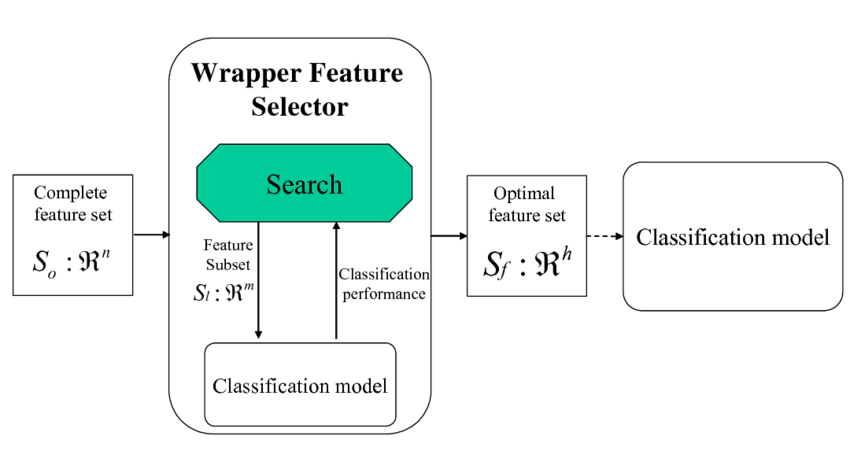
\includegraphics[width=0.85\linewidth]{figuras/wrapper_feature_selector_Baraldi2007.png}
    \caption{Fluxograma de um seletor \textit{wrapper}: geração iterativa de subconjuntos e avaliação por treino/validação do modelo, seguida da seleção do subconjunto ótimo. Adaptado de \cite{Baraldi2007}.}
    \label{fig:wrapper}
\end{figure}

A formulação clássica pode ser expressa como:
\[
S^\ast=\arg\max_{S\subseteq\{1,\dots,p\}} \widehat{M}(S),
\]
em que \(p\) é o número total de atributos e \(\widehat{M}(S)\) é a estimativa empírica do desempenho do modelo com as variáveis em \(S\), tipicamente obtida pela média em \(K\)-\textit{fold} ou por reamostragem \cite{KOHAVI1997273,Dhal2022,Theng2024}. Em aplicações reais, frequentemente se busca não apenas maximizar desempenho, mas também controlar complexidade e interpretabilidade. Isso pode ser operacionalizado por um termo de parcimônia, por exemplo:
\[
S^\ast=\arg\max_{S}\left\{\widehat{M}(S)-\lambda\,|S|\right\},
\]
onde \(|S|\) é a cardinalidade do subconjunto e \(\lambda\ge 0\) controla o compromisso desempenho--parsimonia (em alternativa, trata-se como problema multiobjetivo, buscando soluções com bom desempenho e baixo número de variáveis) \cite{Theng2024,Bouchlaghem2022}. A escolha da métrica \(\widehat{M}\) também não é neutra: em dados desbalanceados, métricas como AUC (Area Under the ROC Curve) e F1 (F1-score) podem ser mais informativas do que acurácia; em regressão, MAE/MSE (Mean Absolute Error/Mean Squared Error)podem ser preferíveis conforme a sensibilidade a outliers; e, em cenários de custo assimétrico, métricas custo-sensíveis são recomendadas para evitar seleção que otimiza um critério desalinhado ao risco operacional \cite{Dhal2022,Theng2024}.

A estratégia de busca é o elemento que torna o \textit{wrapper} viável em espaços grandes, já que a enumeração exaustiva tem custo \(O(2^p\cdot C_{\text{modelo}})\), com \(C_{\text{modelo}}\) representando o custo de treinar/validar o algoritmo \cite{KOHAVI1997273,bolon2018scalability,Emmoh2024}. Na prática, utilizam-se buscas aproximadas como seleção sequencial para frente/trás (SFS/SBS) e variantes \textit{floating}, \textit{best-first} e \textit{beam search}, que exploram o espaço de forma incremental e geralmente produzem bons resultados quando \(p\) é moderado \cite{jovic2015review,Theng2024}. Em modelos específicos, métodos recursivos como RFE são populares por combinarem um critério de importância do modelo com eliminação iterativa; por exemplo, em SVM-RFE, remove-se repetidamente a variável menos relevante segundo a estrutura do classificador, o que frequentemente reduz custo frente a buscas combinatórias e mantém aderência ao avaliador \cite{Theng2024,Bouchlaghem2022}. Para problemas de maior dimensão ou com espaço de busca irregular, meta-heurísticas (p.ex., algoritmos genéticos, PSO, ACO) são amplamente reportadas por fornecerem exploração global com custo controlável, embora sem garantias de otimalidade e com sensibilidade a hiperparâmetros de busca \cite{EBRAHIMIWARKIANI2025129372}. Em seleção não supervisionada (p.ex., clustering), \textit{wrappers} também existem ao substituir a métrica preditiva por índices de qualidade de agrupamento (p.ex., separação/compactação), mas o risco de instabilidade e o custo podem ser ainda mais pronunciados pela ausência de um alvo supervisionado \cite{SolorioFernandez2020}.

O principal custo dos \textit{wrappers} decorre do número de avaliações do modelo durante a busca, o que torna a escalabilidade um problema central em alta dimensionalidade \cite{bolon2018scalability,Emmoh2024}. Na literatura, estratégias recorrentes para reduzir esse custo incluem: (i) restringir o espaço inicial por pré-filtragem (p.ex., remover variáveis constantes, reduzir dimensionalidade por um filtro rápido), preservando o \textit{wrapper} para uma etapa final em espaço menor; (ii) empregar cache/memoização de avaliações para evitar re-treinos redundantes de subconjuntos repetidos; (iii) paralelizar avaliações independentes, o que é particularmente natural quando a busca propõe múltiplos candidatos por iteração; e (iv) adotar aproximações controladas, como validações mais baratas nas fases iniciais (p.ex., menos \textit{folds}) e refinamento posterior nas melhores regiões do espaço \cite{Theng2024,Bouchlaghem2022,de2006parallelizing}. Em cenários modernos, outra prática frequente é combinar \textit{wrappers} com modelos cujo treino seja relativamente eficiente e estável sob diferentes subconjuntos (p.ex., árvores e ensembles), reduzindo \(C_{\text{modelo}}\) e tornando a exploração mais viável \cite{Theng2024,bashir2022novel}.

Do ponto de vista estatístico, o ponto fraco clássico dos \textit{wrappers} é que a própria seleção “\emph{aprende}” a partir do validador interno: quanto mais intensa a busca, maior a probabilidade de \emph{overfitting} ao procedimento de avaliação (seleção otimista), sobretudo quando \(n\) é pequeno e \(p\) é grande \cite{KOHAVI1997273,reunanen2012overfitting,Dhal2022}. Por isso, em experimentos rigorosos, a recomendação é separar claramente o processo de seleção (e eventual ajuste de hiperparâmetros do modelo) da estimativa final de generalização, tipicamente via validação cruzada aninhada (\textit{nested CV}). Nesse arranjo, o laço interno executa a seleção e, se aplicável, a busca de hiperparâmetros; o laço externo fornece uma estimativa menos enviesada do desempenho esperado em dados não vistos \cite{Dhal2022,10.1007/978-3-031-23092-9_12}. Quando a restrição computacional impede \textit{nested CV}, uma alternativa metodológica mínima é reservar um conjunto de teste estritamente intocado até o final e reportar explicitamente a natureza exploratória das escolhas realizadas no treino/validação, evitando conclusões infladas \cite{reunanen2012overfitting,Theng2024}.

Outro aspecto crítico é a estabilidade: como pequenas perturbações na amostra de treino podem alterar o subconjunto selecionado, \textit{wrappers} podem produzir assinaturas distintas com desempenho semelhante, reduzindo interpretabilidade e reprodutibilidade \cite{KHAIRE20221060,somol2010evaluating}. A estabilidade deve ser tratada como um critério de qualidade complementar ao desempenho preditivo, sendo recomendável quantificar a variabilidade do subconjunto via reamostragem (p.ex., repetições de CV ou \textit{bootstrap}) e medir concordância por métricas como Jaccard e índices específicos para seleção de subconjuntos \cite{KHAIRE20221060,somol2010evaluating,BARBIERI2024123667}. Em aplicações em que a interpretabilidade é requisito (p.ex., saúde e finanças), é comum também empregar estratégias \textit{ensemble} de seleção (agregação por frequência de seleção, agregação de rankings ou consenso), que tendem a aumentar robustez e reduzir dependência de uma única partição dos dados \cite{KHAIRE20221060,Theng2024,BARBIERI2024123667}.

Em problemas com dados mistos (numéricos e categóricos), os \textit{wrappers} trazem um desafio adicional: a compatibilidade entre o modelo avaliador, as codificações adotadas (p.ex., \textit{one-hot}, ordinal, \textit{target encoding}) e a medida de desempenho pode induzir vieses na seleção, especialmente quando há alta cardinalidade categórica e assimetria de escalas \cite{SolorioFernandez2022,EBRAHIMIWARKIANI2025129372}. Nesses cenários, a literatura aponta a adoção de abordagens híbridas como caminho pragmático: uma redução inicial por filtros adequados a dados mistos, seguida de \textit{wrapper} restrito em um espaço já “limpo”, preserva parte do ganho preditivo do \textit{wrapper} sem tornar o custo proibitivo \cite{SolorioFernandez2022,EBRAHIMIWARKIANI2025129372,Theng2024}.

\bigskip Os métodos \textit{wrapper} são indicados quando a prioridade absoluta reside na maximização da acurácia preditiva para um indutor específico e há disponibilidade de recursos para sustentar o elevado custo computacional das múltiplas avaliações iterativas \cite{KOHAVI1997273,Theng2024,Emmoh2024}. Todavia, a eficácia dessa abordagem é severamente desafiada em cenários de alta dimensionalidade caracterizados por um número reduzido de amostras frente a uma vasta quantidade de atributos (n << p), situação comum em dados de microarrays onde a busca pode resultar na seleção de correlações espúrias \cite{bolon2018scalability,bashir2022novel,Theng2024}. Essa vulnerabilidade ao \textit{overfitting} no espaço de busca exige salvaguardas rigorosas, sendo imperativo o uso de protocolos de validação cruzada aninhada (\textit{nested CV}) e o reporte transparente dos resultados em conjuntos de teste independentes para evitar estimativas otimistas e enviesadas \cite{reunanen2012overfitting,Dhal2022}. Além disso, quando o objetivo inclui a descoberta de conhecimento, a estabilidade dos atributos selecionados torna-se um critério de avaliação tão crucial quanto o desempenho preditivo, demandando que o subconjunto identificado seja robusto a pequenas perturbações nos dados de treinamento \cite{KHAIRE20221060,BARBIERI2024123667}. Diante de restrições severas de tempo ou complexidade excessiva, a prática mais recomendada consiste na adoção de soluções híbridas que utilizam filtros para uma redução inicial de dimensionalidade antes da busca ou na migração para métodos \textit{embedded}, que oferecem um compromisso mais estável entre eficiência, desempenho e interpretabilidade \cite{Theng2024,EBRAHIMIWARKIANI2025129372,Bouchlaghem2022}.


\subsection{Métodos Embedded}
\label{subsec:embedded}

Os métodos \textit{embedded} realizam a seleção de atributos de forma intrínseca ao processo de aprendizagem, de modo que a identificação das variáveis relevantes emerge diretamente durante o ajuste do modelo. Diferentemente das abordagens \textit{filter}, que são independentes do algoritmo de aprendizagem, e dos métodos \textit{wrapper}, que realizam uma busca externa orientada por avaliação, os métodos \textit{embedded} incorporam mecanismos de penalização, regularização ou critérios de importância diretamente na função objetivo do modelo. Essa integração permite que a seleção ocorra concomitantemente ao treino, reduzindo a necessidade de etapas externas de seleção e mitigando o elevado custo computacional associado a estratégias de busca explícita \cite{10.1007/978-3-031-23092-9_12,Theng2024,Dhal2022}. Em virtude desse equilíbrio entre eficiência computacional e capacidade de capturar interações entre atributos, estudos recentes apontam os métodos \textit{embedded} como particularmente adequados a pipelines de produção e a cenários de aplicação prática em larga escala \cite{EBRAHIMIWARKIANI2025129372,Bouchlaghem2022,Emmoh2024}.

Do ponto de vista formal, uma formulação canônica dos métodos \textit{embedded} baseados em regularização pode ser expressa como um problema de otimização no qual se busca minimizar a soma entre uma função de perda empírica e um termo de penalização:
\[
\widehat{\beta} \;=\; \arg\min_{\beta}\; \mathcal{L}(y, X\beta) + \lambda\,\Omega(\beta),
\]
em que $\mathcal{L}$ representa a perda empírica (por exemplo, MSE ou \textit{log-loss}), $\Omega(\beta)$ corresponde ao termo de regularização e $\lambda>0$ controla a intensidade da penalização. As instâncias mais consolidadas dessa abordagem incluem o LASSO, baseado em penalização $L_1$, o Ridge, baseado em penalização $L_2$, e o ElasticNet, que combina ambas. O LASSO promove esparsidade explícita ao zerar coeficientes associados a atributos irrelevantes, o Ridge atua predominantemente na redução da variância sem induzir seleção direta, enquanto o ElasticNet apresenta-se como uma solução intermediária, particularmente eficaz em cenários com alta correlação entre atributos \cite{Theng2024,10.1007/978-3-031-23092-9_12,Dhal2022}. Revisões recentes destacam o papel central desses métodos em problemas tabulares e de alta dimensionalidade, sobretudo quando a interpretabilidade dos coeficientes é um requisito relevante \cite{BARBIERI2024123667,KHAIRE20221060}.

Além dos modelos lineares penalizados, uma classe amplamente utilizada de métodos \textit{embedded} corresponde aos algoritmos não lineares baseados em árvores de decisão e em ensembles. Estruturas como \textit{Decision Trees}, \textit{Random Forests} e métodos de \textit{Gradient Boosting} incorporam mecanismos nativos de avaliação da importância dos atributos, geralmente derivados do ganho de impureza associado às divisões internas do modelo. Essas medidas permitem que tais algoritmos sejam utilizados como seletores \textit{embedded} sem a necessidade de procedimentos adicionais de busca. Entretanto, a literatura aponta que importâncias baseadas exclusivamente em ganho de impureza podem introduzir vieses, favorecendo variáveis com maior número de níveis ou maior variância. Em razão disso, medidas alternativas, como \textit{permutation importance}, bem como variantes regularizadas de ensembles, são frequentemente recomendadas para análises interpretativas mais robustas \cite{SolorioFernandez2020,SolorioFernandez2022,EBRAHIMIWARKIANI2025129372,Theng2024}. Avaliações comparativas indicam ainda que métodos baseados em árvores tendem a apresentar maior estabilidade em dados mistos, embora se beneficiem significativamente da combinação com técnicas de permutação e validação externa \cite{Bouchlaghem2022,Emmoh2024}.

No que se refere às suas propriedades práticas, os métodos \textit{embedded} apresentam vantagens recorrentes destacadas na literatura, entre as quais se incluem a realização da seleção durante o próprio treino do modelo, a redução do custo computacional quando comparados a abordagens \textit{wrapper} e a facilidade de integração em fluxos automatizados de validação, como a validação cruzada. Tais características tornam esses métodos particularmente atraentes em ambientes de produção e aplicações industriais \cite{Theng2024,Dhal2022,10.1007/978-3-031-23092-9_12}. Todavia, essas vantagens coexistem com limitações bem documentadas. A seleção resultante é fortemente dependente do modelo e do tipo de regularização empregado, podendo variar substancialmente entre diferentes algoritmos. Ademais, em contextos de alta correlação entre atributos, métodos como o LASSO tendem a selecionar variáveis de forma arbitrária, o que pode comprometer a estabilidade do subconjunto selecionado. Esse problema é agravado em cenários de alta dimensionalidade com baixo número de amostras ($n \ll p$), bem como pela presença de vieses específicos nas medidas de importância utilizadas por modelos baseados em árvores \cite{KHAIRE20221060,BARBIERI2024123667,EBRAHIMIWARKIANI2025129372,Theng2024}.

Sob a perspectiva de complexidade e escalabilidade, o desempenho dos métodos \textit{embedded} varia conforme o algoritmo subjacente. Modelos de regressão penalizada, quando implementados com técnicas eficientes de otimização, como \textit{coordinate descent} ou métodos proximais, apresentam boa escalabilidade mesmo em cenários de alta dimensionalidade. Por outro lado, ensembles de árvores demandam recursos computacionais proporcionais ao número de estimadores e à profundidade média das árvores, embora possam ser acelerados por implementações distribuídas amplamente adotadas na prática, como XGBoost e LightGBM. Em problemas com espaços de atributos extremamente grandes, a literatura recomenda a combinação de uma pré-filtragem leve por exemplo, remoção por baixa variância ou alta correlação com métodos \textit{embedded}, bem como o uso de \textit{early stopping}, ajuste automático do parâmetro de regularização via \textit{nested cross-validation} e estratégias de \textit{caching} para viabilizar experimentos em larga escala \cite{Theng2024,Bouchlaghem2022,Emmoh2024,10.1007/978-3-031-23092-9_12}.

Estudos recentes enfatizam que a avaliação empírica de métodos \textit{embedded} não deve se restringir ao desempenho preditivo, sendo imprescindível quantificar a estabilidade dos subconjuntos selecionados. Recomenda-se a execução de múltiplas reamostragens, por meio de \textit{bootstrap} ou validação cruzada repetida, e a utilização de métricas específicas de estabilidade, como os índices de Jaccard e Kuncheva, complementadas por análises de \textit{permutation importance} em conjuntos de validação externos. Evidências empíricas sugerem que o ElasticNet frequentemente apresenta um compromisso mais favorável entre esparsidade e estabilidade quando comparado ao LASSO puro, enquanto métodos baseados em árvores, quando combinados com testes de permutação, produzem estimativas de importância mais confiáveis em dados heterogêneos \cite{KHAIRE20221060,BARBIERI2024123667,SolorioFernandez2022,EBRAHIMIWARKIANI2025129372}.

Para assegurar validade, reprodutibilidade e interpretabilidade dos resultados, a literatura converge para um conjunto de boas práticas experimentais que incluem a documentação rigorosa das etapas de pré-processamento, o ajuste criterioso dos hiperparâmetros de regularização por meio de \textit{nested cross-validation}, a combinação de coeficientes ou importâncias internas com métodos baseados em permutação quando a interpretabilidade for um objetivo central, e o reporte conjunto de métricas de desempenho, estabilidade e custo computacional. A adoção sistemática dessas práticas é fundamental para permitir comparações justas entre métodos \textit{embedded} e consolidar sua aplicação em contextos científicos e industriais \cite{Dhal2022,Theng2024,Bouchlaghem2022,10.1007/978-3-031-23092-9_12}.
A Figura~\ref{fig:embedded} ilustra o funcionamento geral dos métodos \textit{embedded}, evidenciando que a geração do subconjunto de atributos e a avaliação do desempenho preditivo ocorrem de forma integrada ao processo de aprendizagem, em contraste com abordagens baseadas em busca externa.


\begin{figure}[htbp]
    \centering
    \includegraphics[width=0.85\linewidth]{figuras/embedded.png}
    \caption{Procedimento \textit{Embedded}: seleção de atributos integrada ao treino do modelo (adaptado de \cite{10.1007/978-3-031-23092-9_12}).}
    \label{fig:embedded}
\end{figure}


\subsection{Métodos Híbridos}\label{subsec:hibridos}

Os métodos híbridos surgem como uma solução estratégica na seleção de atributos, visando superar as limitações individuais das abordagens de filtro e \textit{wrapper} ao buscar um ponto de equilíbrio ideal entre eficiência computacional e precisão preditiva \cite{EBRAHIMIWARKIANI2025129372,10895909}. Essa classe de algoritmos aproveita a velocidade e a escalabilidade inerentes aos filtros para realizar um peneiramento inicial dos dados, eliminando atributos irrelevantes e reduzindo drasticamente o espaço de busca antes da aplicação de uma avaliação mais rigorosa e custosa \cite{EBRAHIMIWARKIANI2025129372,10895909}. Ao integrar essas capacidades, os métodos híbridos conseguem capturar interações complexas entre variáveis que seriam ignoradas por filtros univariados, mantendo um custo computacional significativamente menor do que o exigido por métodos \textit{wrapper} puros \cite{EBRAHIMIWARKIANI2025129372,10895909}.

O fluxo operacional dessa categoria é caracterizado por um processo em dois estágios principais, conforme ilustrado na Figura \ref{sym14101955} \cite{sym14101955}. No primeiro estágio, o conjunto original de atributos é submetido a um método de filtro (baseado em critérios estatísticos ou de teoria da informação) para realizar uma redução inicial de dimensionalidade, eliminando ruídos e redundâncias para gerar um \textit{ranking} ou um subconjunto reduzido \cite{sym14101955}. No segundo estágio, um algoritmo de otimização atuando como um \textit{\textbf{wrapper}} conduz uma busca fina no espaço de estados para identificar a combinação ótima de variáveis para um indutor ou classificador específico \cite{sym14101955}. Essa arquitetura híbrida permite que o processo de seleção se beneficie da inteligência de algoritmos metaheurísticos, como Algoritmos Genéticos (GA), Otimização por Enxame de Partículas (PSO) ou Colônia de Formigas (ACO), para navegar de forma robusta no espaço de hipóteses, evitando mínimos locais e reduzindo o custo computacional em comparação com métodos \textit{wrapper} puros \cite{sym14101955, EBRAHIMIWARKIANI2025129372, 10895909}.

\begin{figure}[htbp]
    \centering
    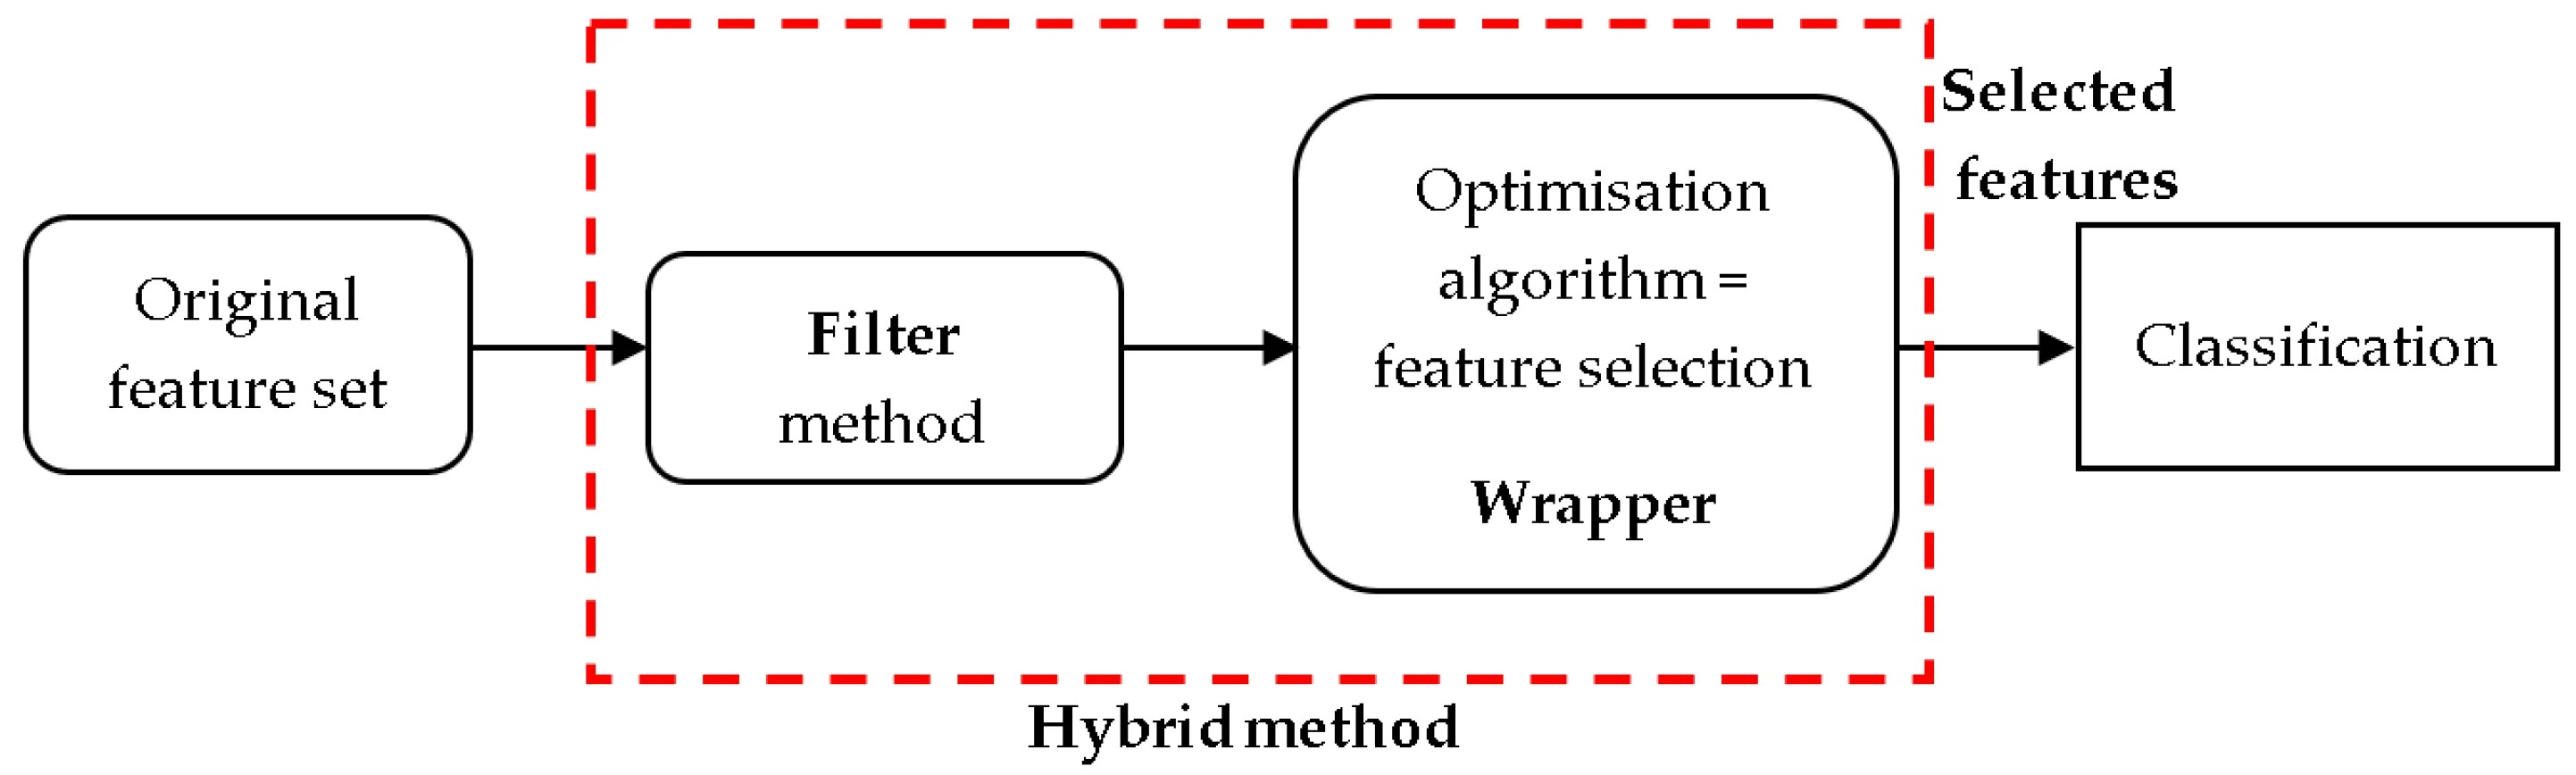
\includegraphics[width=1\linewidth]{figuras/hibrido.jpg}
    \caption{Fluxo de trabalho de um método híbrido combinando filtro e \textit{wrapper}. Fonte: \cite{sym14101955}.}
    \label{sym14101955}
\end{figure}

A adoção de modelos híbridos é particularmente vantajosa em cenários de alta dimensionalidade, onde a presença de ruído e redundância pode deteriorar severamente a capacidade de generalização dos modelos de aprendizagem \cite{villar2022reduccao, salhi2025optimizing, ferreira2014feature}. Ao combinar diferentes estratégias de avaliação, essa abordagem promove uma maior estabilidade na seleção de atributos, garantindo que o subconjunto identificado seja menos sensível a pequenas perturbações nos dados de treinamento e apresente um viés reduzido \cite{villar2022reduccao, salhi2025optimizing}. Essa robustez é fundamental para a descoberta de conhecimento em domínios críticos, onde a interpretabilidade das variáveis escolhidas é tão relevante quanto a acurácia de classificação final \cite{salhi2025optimizing}.

Em última análise, a hibridização permite uma personalização profunda do processo de seleção de atributos de acordo com as necessidades específicas do problema em mãos e dos recursos computacionais disponíveis \cite{sym14101955,BARBIERI2024123667}. Ao gerenciar de forma dinâmica o \textit{trade-off} entre a exploração do espaço de busca e o tempo de execução, os métodos híbridos consolidam-se como uma das ferramentas mais eficazes para lidar com as complexidades crescentes do \textit{Big Data} e dos conjuntos de dados multimodais \cite{bolon2018scalability,EBRAHIMIWARKIANI2025129372,SolorioFernandez2022}. Essa integração contínua de métodos estatísticos com técnicas de busca baseadas em desempenho direto permite que o sistema de aprendizagem identifique os atributos mais informativos, maximizando a acurácia global e minimizando o risco de sobreajuste \cite{sym14101955,BARBIERI2024123667,EBRAHIMIWARKIANI2025129372,SolorioFernandez2022}.
